\documentclass{siproblemset}

% SI Session Information
\course{MTH 1321}       % the course of your SI
\sessionnum{10}          % (optional) specify the session number
\sessiondate{2/24/22}   % the date of the session

\warmup{Concept Review}
\topic{Rates of Change}
\topic{Higher Derivatives}
\topic{Trigonometric Derivatives}
\cooldown{Graphs of Derivatives}

% Worksheet Information
\title{Higher Derivatives}
\sections{Sections 3.5}
\withnamespace

\begin{document}
    \maketitle
    
    \activity{Warmup}{Concept Review}{Try these problems \textbf{alone} as your peers join the session. Do your best to not refer to your notes.}{15 minutes}

    \frq{What is the mathematical relationship between position, velocity, acceleration, and speed?}
    \smallspace
    \mcq[2]{Evaluate the following:}{
        \task $\dddx \left[ c\right] $
        \task $\dddx \left[ x^k\right] $
        \tinysp
        \task $\dddx \left[cf(x)\right]$
        \task $\dddx \left[ f(x)\pm g(x)\right] $
        \tinysp
        \task $\dddx \left[ e^{kx}\right] $
        \tinysp
        \task $\dddx \left[f(x)\cdot g(x)\right]$
        \task $\dddx \left[ \sqrt{x}\right] $
        \tinysp
        \task $\dddx \left[x\right]$
        \task $\dddx \left[ \dfrac1x\right] $
        \tinysp
        \task $\dddx \left[ \dfrac{f(x)}{g(x)}\right] $
    }
    
    \pagebreak
    
    \activity{Activity 1}{Higher-Order Derivatives}{Work together in your \textbf{breakout rooms} to answer these questions. Do your best to not refer to your notes while working on these problems.}{30 minutes}
    
    \mcq{Find $f'(x)$, $f''(x)$, and $f'''(x)$.}{
        \task{$f(x)=2x^3-3x^2+2x-e^{2x}$}
        \mediumspace
        \task{$f(x)=3e^x-x^3$}
        \mediumspace
        \task{$f(x)=\dfrac{1}{x}$}
        \mediumspace
        \task{$f(x)=(2x+1)(x^2-2)$}
        \mediumspace
        \task{$f(x)=\pi^2(x-1)$}
        \mediumspace
        \task{$f(x)=x^5e^x$ (only compute $f'$ and $f''$)}
        \mediumspace
    }
    \pagebreak
    
    \activity{Activity 2}{Differential Equations}{Work together in your \textbf{breakout rooms} to answer these questions. Do your best to not refer to your notes while working on these problems.}{30 minutes}
    
    \frq{Show that $y=x^2+2x+1$ is a solution to the differential equation}
    $$xy''=y'-2$$
    \Largesp
    \frq{Find all values of $n$ such that $y=x^n$ is a solution of}
    $$xy''+4\frac{y}{x}=4y'$$
    \pagebreak

    \activity{Cooldown}{Graphs of Derivatives}{Try these problems \textbf{alone}. Do your best to not refer to your notes.}{15 minutes}
    
    \begin{multipartquestion}
        Given the graph of $s$ below, which represents the height (in feet) of a particle as a function of time $t$ (in seconds), determine which of the other three graphs represent its velocity and acceleration over the same time interval.
        
        \begin{multicols}{2}
            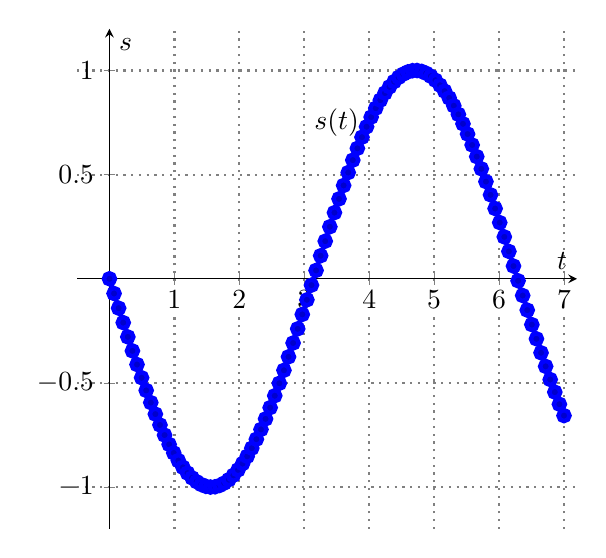
\begin{tikzpicture}
            \begin{axis}[axis x line=center, axis y line=middle,
            width=2.5in, height=2.5in, 
            scale only axis, %axis equal,
            xmin=-0.5, xmax=7.2,
            ymin=-1.2, ymax=1.2,
            xtick={0,...,7}, ytick={-1,-0.5,...,1},
            xticklabel style={draw=none, inner sep=2pt, fill=white, text opacity=1},
            xlabel={$t$}, ylabel={$s$},
            grid=both, grid style={line width=.8pt, draw=gray, dotted},
            minor tick num=0, 
            samples=100]
            \addplot+[blue, ultra thick, domain=0:7] {-sin(x*180/pi)};
            \node at (3.5, 0.75) {$s(t)$};
            \end{axis}
            \end{tikzpicture}
            \tinysp
            
            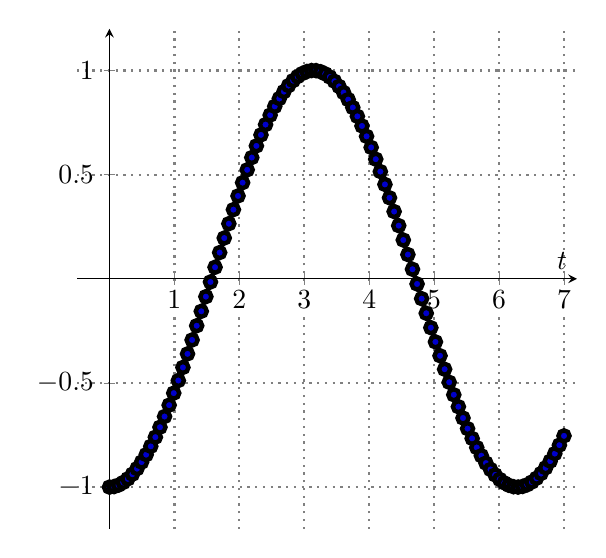
\begin{tikzpicture}
            \begin{axis}[axis x line=center, axis y line=middle,
            width=2.5in, height=2.5in, 
            scale only axis, %axis equal,
            xmin=-0.5, xmax=7.2,
            ymin=-1.2, ymax=1.2,
            xtick={0,...,7}, ytick={-1,-0.5,...,1},
            xticklabel style={draw=none, inner sep=2pt, fill=white, text opacity=1},
            xlabel={$t$}, ylabel={},
            grid=both, grid style={line width=.8pt, draw=gray, dotted},
            minor tick num=0, 
            samples=100]
            \addplot+[black, ultra thick, domain=0:7] {-cos(x*180/pi)};
            \end{axis}
            \end{tikzpicture}
            
            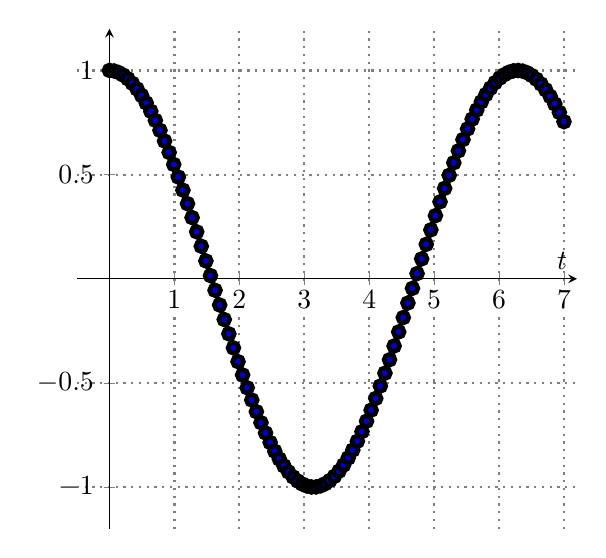
\begin{tikzpicture}
            \begin{axis}[axis x line=center, axis y line=middle,
            width=2.5in, height=2.5in, 
            scale only axis, %axis equal,
            xmin=-0.5, xmax=7.2,
            ymin=-1.2, ymax=1.2,
            xtick={0,...,7}, ytick={-1,-0.5,...,1},
            xticklabel style={draw=none, inner sep=2pt, fill=white, text opacity=1},
            xlabel={$t$}, ylabel={},
            grid=both, grid style={line width=.8pt, draw=gray, dotted},
            minor tick num=0, 
            samples=100]
            \addplot+[black, ultra thick, domain=0:7] {cos(x*180/pi)};
            \end{axis}
            \end{tikzpicture}
            \tinysp
            
            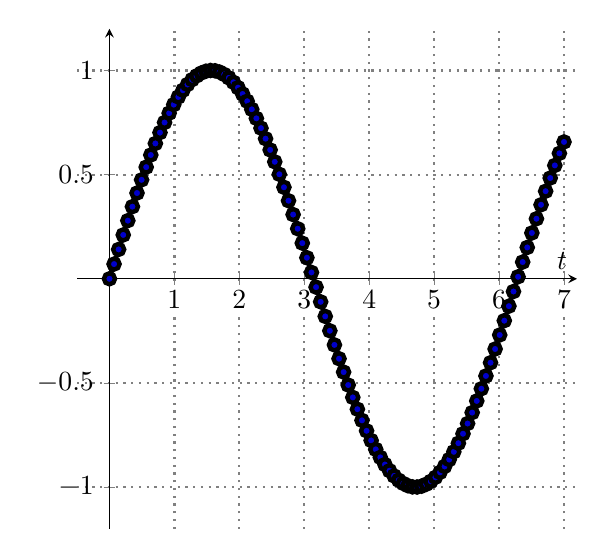
\begin{tikzpicture}
            \begin{axis}[axis x line=center, axis y line=middle,
            width=2.5in, height=2.5in, 
            scale only axis, %axis equal,
            xmin=-0.5, xmax=7.2,
            ymin=-1.2, ymax=1.2,
            xtick={0,...,7}, ytick={-1,-0.5,...,1},
            xticklabel style={draw=none, inner sep=2pt, fill=white, text opacity=1},
            xlabel={$t$}, ylabel={},
            grid=both, grid style={line width=.8pt, draw=gray, dotted},
            minor tick num=0, 
            samples=100]
            \addplot+[black, ultra thick, domain=0:7] {sin(x*180/pi)};
            \end{axis}
            \end{tikzpicture}
        \end{multicols}
    \end{multipartquestion}

    \frq{What is the derivative of $f(x)=x^2\cot(x)$?}
\end{document}